%
% Lecture Template for ME3001-001-Tristan Hill - Spring 2020
% Mechanical Engineering Analysis with MATLAB
% Ordinary Differential Equations - Lecture 5
% Solving Second Order ODEs with the Trial Solution Method
% 

% Document settings

\documentclass[fleqn]{beamer}                  % for presentation ?
%\documentclass[handout]{beamer}  % for handout ?
\usepackage{beamerthemesplit}
\usepackage{amsmath}
\usepackage{listings}
\usepackage{multicol}

\beamertemplateballitem

\definecolor{TTUpurple}{rgb}{0.3098, 0.1607, 0.5176} % TTU Purple (primary)
\definecolor{TTUgold}{rgb}{1.0000, 0.8666, 0.0000} % TTU Gold (primary)

\setbeamercolor{palette primary}{bg=TTUpurple,fg=TTUgold}
\setbeamercolor{palette secondary}{bg=black,fg=TTUgold}
\setbeamercolor{palette tertiary}{bg=black,fg=TTUpurple}
\setbeamercolor{palette quaternary}{bg=TTUgold,fg=black}
\setbeamercolor{structure}{fg=TTUpurple} % itemize, enumerate, etc
\setbeamercolor{section in toc}{fg=TTUpurple} % TOC sections

%\usefonttheme{professionalfonts}

\newcommand{\LNUM}{3\hspace{2mm}} % Lecture Number 
\newcommand{\secondtitle}{Trial Solution for Second Order ODEs}% second line of the title of this presentation , aka the topic of this lecture
\newcommand{\vspcc}{\vspace{6mm}\\ } 
\newcommand{\vspc}{\vspace{3mm}\\} 
\newcommand{\hspc}{\hspace{5mm} } 

\newcommand{\sectiontitleI}{Trial Solution Method} % More Titles and Stuff
\newcommand{\sectiontitleII}{Complementary Solution}
\newcommand{\sectiontitleIII}{Particular Solution}
\newcommand{\sectiontitleIV}{Apply Initial Conditions}


\title{\vspace{2mm}\\Ordinary Differential Equations - Lecture \LNUM}
\author{ME3001 - Mechanical Engineering Analysis} % original formatting from Mike Renfro, September 21, 2004

\date{Mechanical Engineering\vspc Tennessee Technological University}

\begin{document}

\lstset{language=MATLAB,basicstyle=\ttfamily\small,showstringspaces=false}



\frame{\titlepage \center\textbf{\secondtitle}\vspcc}

% Section 0 - Outline
\frame{
	
	{\bf Lecture \LNUM - \secondtitle:} \vspace{3mm}\\ % ' topics' are beamer 'sections' - TWH
	
	\begin{itemize}
	
		\item \sectiontitleI    \vspc % Section I
		\item \sectiontitleII 	\vspc % Section II
		\item \sectiontitleIII 	\vspc %Section III
		\item \sectiontitleIV 	\vspc %Section IV
	
	\end{itemize}

}


% Section I
\section{\sectiontitleI}

	% Section I - Frame I
	\frame{ \small
		\frametitle{\sectiontitleI}

\frametitle{Trial Solution Method}
Use the {\bf trial solution method} to solve the ODE. \vspace{2mm}\\
This is an {\bf analytical} method that you learned in calculus but it may have been called something different. In the Zill book it is called {\it Homogenous Linear ... Constant Coefficients (4.3-4.4)}. \vspcc

\[a_2y''+a_1y'+a_0y=f(x)\] \vspcc


	}
	
	% Section I - Frame II
	\frame{
		\frametitle{\sectiontitleI}

				    

	}

% Section II
\section{\sectiontitleII}
	
	% Section II - Frame I
	\frame{ \small
		\frametitle{\sectiontitleII}

\underline{Step 1} - Find the {\bf complementary part} of the solution from the \vspace{1mm}\\ left hand side of the ODE alone (LHS=0). \\

\[a_2y''+a_1y'+a_0y=f \hspace{5mm}\rightarrow\hspace{5mm} a_2y''+a_1y'+a_0y=0\] \\

Assume an exponential solution for the complementary part. \[y_{complementary}=y_c(t)=\] \\

Substitute this solution into the ODE (LHS=0).
	}
		
	% Section II - Frame II
	\frame{ 
		\frametitle{\sectiontitleII}
	
	}



% Section III
\section{\sectiontitleIII}
	
	% Section III - Frame I
	\frame{ \small
		\frametitle{\sectiontitleIII}

\underline{Step 2} - Find the {\bf particular part} of the solution from the entire equation (LHS=RHS). \vspcc  
\[a_2y''+a_1y'+a_0y=f\] \\

The {\it form of the particular part} follows the RHS of  the ODE. \vspc

\[y_{particular}=y_p(t)=\]  \\

Substitute this solution into the ODE above and solve for any unknown constants in $ y_p(t) $. 
		}
		
		% Section III - Frame II
	\frame{ 
		\frametitle{\sectiontitleIII}
	
	}

		
% Section IV:
\section{\sectiontitleIV}

	% Section IV - Frame I
	\frame{ \small
		\frametitle{\sectiontitleIV}

\underline{Step 3} - Now combine the {\bf complementary} and {\bf particular} solutions through {\it superposition}. \\

\[y(x)=y_c(x)+y_p(x)=\] \\

The ODE is first order and we have \underline{\hspace{10mm}} unknown. Coincidence?\vspcc

\[y(x)=\]  \\

This {\bf initial value problem} requires \underline{\hspace{10mm}} intial condition.\vspace{2mm}\\

	}

	% Section IV - Frame II
	\frame{ \small
		\frametitle{\sectiontitleIV}
	

\[y(x=0)=\] 
\[y'(x=0)=\] 

\vspace{40mm}

}
	% Section IV - Frame II
	\frame{ \small
		\frametitle{\sectiontitleIV}
	What does the solution look like this time?\\

\[y(x)=\] \\

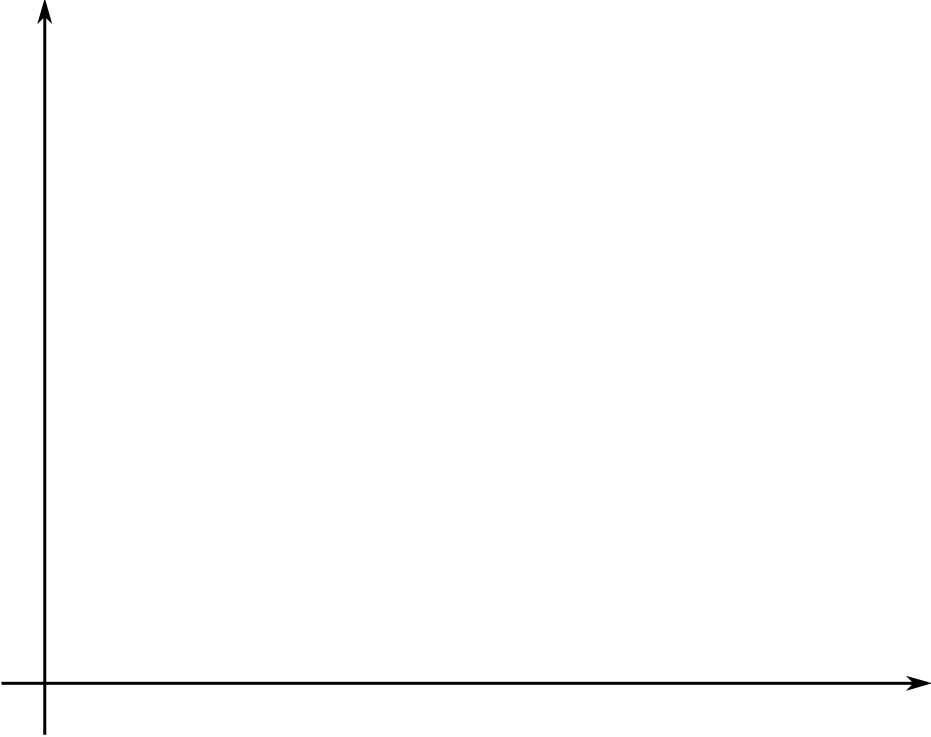
\includegraphics[scale=0.15]{lecture1_fig2.png}\hspace{5mm} 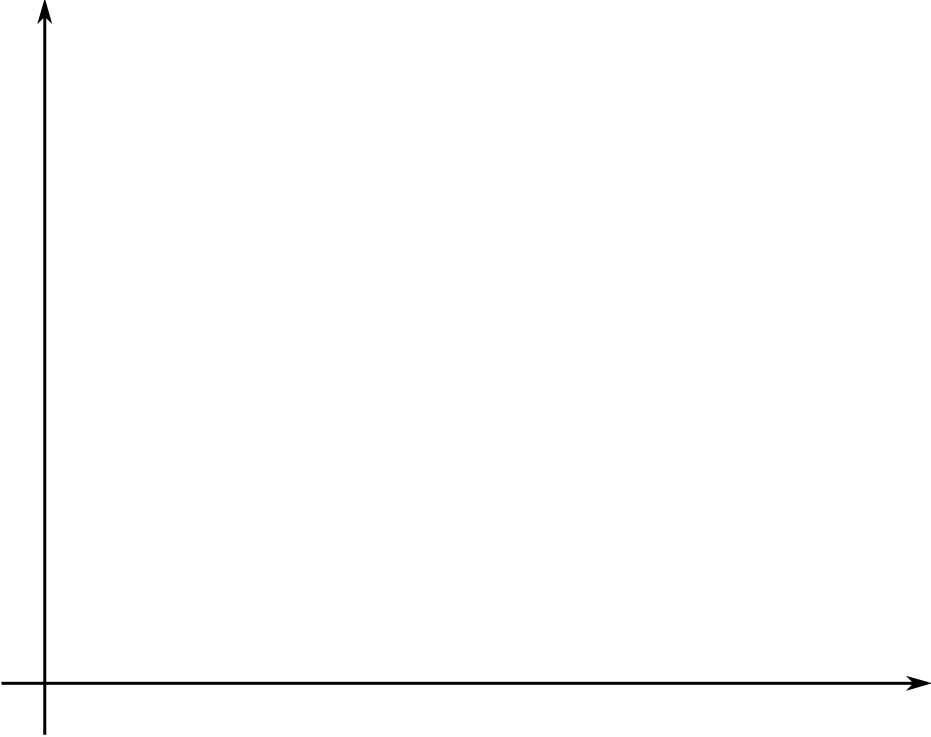
\includegraphics[scale=0.15]{lecture1_fig2.png}
}
\end{document}
